%!TEX root=../../root.tex

\section{Lezione 17}

\subsection{Teoria della complessità}

Ha senso parlare di complessità solo riguardo quei linguaggi che sono decisi da $MdT$. Per questi, a parità di lunghezza della stringa di input, l'esecuzione può richiedere tempi molto diversi.

\begin{description}
\item \textit{esempio}: 
\begin{enumerate}
\item data la macchina $T_{1}$ per il linguaggio $L(T_{1}) = \{0^n1^n \ | \ n \geq 0\}$ 
\item per un input ben formato $0^n1^n$ la distanza tra uno $0$ e il suo $1$ corrispondente sarà al più $n$. L'algoritmo risolutivo compie approssimativamente $n$ passi per ogni coppia di $0$ e $1$ da marcare, quindi siamo nell'ordine di $O(n^2)$
\item per un input mal formato, ad esempio $10^n$, termina in $O(1)$
\end{enumerate}
\end{description}

\subparagraph{Funzione tempo di $T$}

Data una $T \in DTM$ che si ferma sempre definiamo la funzione tempo di $T$
\[
	t_{T}(n) = \text{ max\{numero di mosse eseguite da T su un input di dimensione n\} } 
\]
\begin{description}
\item \textit{esempio}:
in riferimento al problema $T_{1}$ visto in precedenza, $t_{T_{1}}(n) = O(n^2)$
\end{description}

Possiamo quindi definire la classe dei linguaggi decisi da una DTM in tempo $O(n^k)$ come
\[
	TIME(n^k) =  \{ L \ | \ T \in DTM \ e \  L(T) = L \ e \ t_{T}(n) = O(n^k) \}
\]

\subparagraph{Funzione spazio di $T$}

Data una $T \in DTM$ che si ferma sempre definiamo la funzione spazio utilizzato (calcolato nel numero di celle di nastro) di $T$
\begin{gather*}
	S_{T}(n) = max\{\text{numero di celle del nastro impiegate in una computazione } \\
	\text{su un input di lunghezza }n\}
\end{gather*}
\begin{description}
\item \textit{esempio}:
in riferimento al problema $T_{1}$ visto in precedenza, $S_{T_{1}}(n) = O(n)$
\end{description}

\subparagraph{$t_{T}(n)$ limita superiormente $S_{T}(n)$}

Sotto l'ipotesi che almeno in un caso tutto l'input sia letto, possiamo limitare superiormente lo spazio $S_{T}(n)$ con il tempo $t_{T}(n)$, infatti ad ogni passo posso scrivere al più una cella.
\[
	n \leq S_{T}(n) \leq t_{T}(n)
\]

\subparagraph{$S_{T}(n)$ limita superiormente $t_{T}(n)$} 

Conoscendo $S_{T}(n)$ posso limitare superiormente $t_{T}(n)$ analizzando le configurazioni. Il numero delle configurazioni ottenibili, sotto l'ipotesi che in ogni computazione la porzione di nastro impegnata è proprio $S_{T}(n)$ è definito come segue:
\[
	\text{Hyp: } \ |\alpha a \beta | = S_{T}(n)
\]
Le possibili configurazioni sono quindi
\[
	S_{T}(n)  | \Gamma |^{S_{T}(n)}  |Q|
\]
dove $S_{T}(n)$ sono le possibili posizioni della testina; $| \Gamma |^{S_{T}(n)}$ sono tutte le possibili stringhe scrivibili su nastro e $|Q|$ il numero degli stati della $MdT$.

\[
	2^{\log|Q|} \big( 2^{\log|\Gamma|} \big)^{S_{T}(n)} 2^{\log S_{T}(n)} = 2^{\log|Q| + \log|\Gamma|S_{T}(n) + \log S_{T}(n) } = 2^{O(S_{T}(n))}
\]
\[
	t_{T}(n) \leq 2^{O(S_{T}(n))}
\]

\subsection{Tempi di calcolo su diversi modelli di MdT}

Data $T \in  TM_{k}$ cosa possiamo dire delle funzioni $t_{T}(n)$ e $S_{T}(n)$?
La definizione di $t_{T}(n)$ resta invariata. Cambia invece $S_{T}(n)$:
\begin{gather*}
S_{T}(n) = \text{ \{somma dei massimi, per ognuno dei k nastri,} \\ \text{del numero di celle del nastro impiegate in una computazione su un input di lunghezza n\} }
\end{gather*}

\begin{description}
\item \textit{esempio}:
Avendo $T \in  TM_{k}$ con un $t_{T}(n)$ definito, e data una $T^{1} \in  TM$ tale che $L(T) = L(T^{1})$, cosa possiamo dire di $t_{T^{1}}(n)$ e $S_{T^{1}}(n)$?

\begin{enumerate}
\item $S_{T^{1}}(n) = O(t_{T}(n))$
\item Per definire $t_{T}(n)$ devo simulare ogni mossa di $T$ in $T^{1}$, il che richiede un numero costante $t_{T}(n)$ di scansioni del nastro, e ogni scansione richiede al più $t_{T}(n)$ passi. Ne segue che $t_{T^{1}}(n) = O(t_{T}^{2}(n))$
\end{enumerate}

\end{description}

\subsection{La classe P}
Definisco $P$, la classe di tutti i linguaggi decisi in tempo polinomiale (e che sono definiti quindi "trattabili") da una TM.
\[
	P = \{ L \ | \ \exists T \in TM, L(T) = L \ e \ t_{T}(n) = O(n^k) \  \forall k \geq 0 \}
\]
\[
	P = \bigcup_{k \geq 0} TIME(n^k)
\]

$P$ è importante in quanto:
\begin{enumerate}
\item E' invariante per tutti i modelli di computazione polinomiali equivalenti alla MdT deterministica a singolo nastro, e
\item $P$ corrisponde alla classe di problemi che sono realisticamente risolvibili da un computer.
\end{enumerate}
\subparagraph{Tesi Cobham-Edmonds} Definiamo \textbf{trattabili} tutti i problemi polinomialmente risolvibili. E \textbf{intrattabili} tutti i problemi che si risolvono con algoritmi esponenziali. Non tutti i problemi cadono in queste due categorie, infatti esistono problemi per i quali non si conosce un algoritmo polinomiale ma non è stato dimostrato che siano intrattabili.\\ A sostegno di questa tesi abbiamo la stabilità di $P$, ossia che un problema in $P$ è polinomiale in qualsiasi modello di calcolo. Contro questa tesi abbiamo il fatto che quando il grado del polinomio supera il quarto grado i problemi non sono più trattabili.
\subsection{Esempi di problemi in P}

\subparagraph{$PATH$ è in P} 

\begin{gather*}
PATH = \{ <G,s,t> | \text{ G è un grafo diretto (orientato) e s e t} \\ \text{sono due suoi vertici, trai i quali esiste un cammino} \}
\end{gather*}
\[
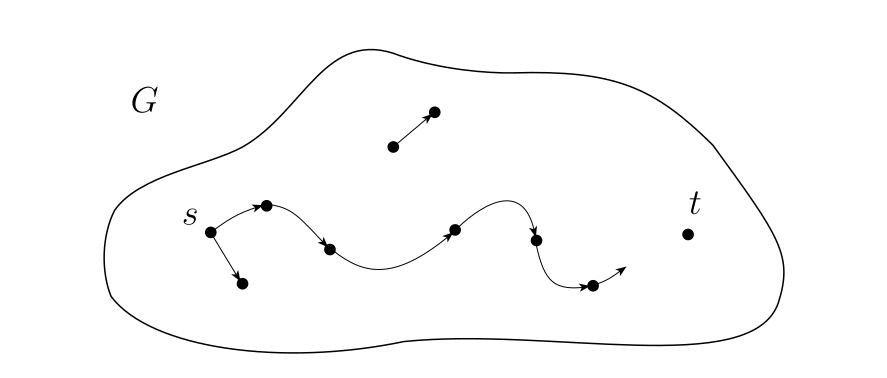
\includegraphics[scale=0.30]{path}
\]
\begin{description}
\item \textit{algoritmo}: 
input $<G,s,t>$
output $si$ se $<G,s,t> \in PATH$, $no$ altrimenti
\begin{enumerate}
\item $M = \{ s \}$
\item cicla fin quando non aggiungo più vertici:
\item \ \ \ \ $M \cup \{ V \ | \ (x, V) \in E, \ x \in M \}$
\item se $t \in M$, rispondo $si$, $no$ altrimenti
\end{enumerate}
\end{description}

\begin{description}
\item \textit{complessità}:
Analizziamo l'algoritmo e mostriamo che ha complessità polinomiale. Il punto 1 e 4 sono eseguiti una sola volta. Il passo 3 è eseguito al più $|V|$ volte. Il numero di esecuzioni delle fasi è quindi al più $1 + 1 + |V|$, quindi polinomiali nella grandezza di $G$. I passi 1 e 4 sono facilmente implementabili in tempo polinomiale. Il passo 3 involve una scansione dell'input e un test per vedere se un vertice è già stato marcato, il che è facilmente implementabile in tempo polinomiale. Quindi $PATH \in P$.
\end{description}

\subparagraph{$E_{DFA}$ è in P} 
\begin{gather*}
E_{DFA} = \{ <A> | A \in DFA \ e \ L(A)=\emptyset \}
\end{gather*}
Per $A \in DFA$ si ha $L(A)=\emptyset$ quando non vi è un cammino dal suo stato di inizio $q_0$ ad un suo stato di accettazione $q_F$. Potendo determinare in tempo polinomiale l'insieme $PATH$ dei nodi per i quali esiste un cammino in $G$, ne concludiamo che potremo calcolare l'insieme $\overline{E_{DFA}}$ in tempo polinomiale, riducendolo al problema $PATH$.
\[
	\overline{E_{DFA}} \leq_{m} PATH
\]

\subsection{Determinare il rifiuto di una NTM}
Data una $T \in  NTM$ che si ferma sempre, definisco una strategia che verifica il rifiuto da parte di $T$ di un dato input $x$. 
Come nell'algoritmo studiato per dimostrare l'equivalenza tra $TM$ e $NTM$, simuliamo la macchina non deterministica $T$, che per ipotesi diciamo avere come grado di non determinismo 2 (e quindi un albero delle configurazioni binario), con una deterministica $T' \in TM$ utilizzando i tre nastri: input, lavoro, guida. Aggiungo questa volta un ulteriore nastro, detto di conteggio. Questo nastro terrà il conto del numero di foglie nell'albero delle configurazioni di $T$ che hanno una configurazione di rifiuto o per cui la configurazione è bloccata. Al termine della simulazione di $T$, se il valore numerico nel nastro di conteggio è uguale a $2^h$, con $h$ altezza dell'albero, allora tutte le foglie sono o di rifiuto o bloccate. Di conseguenza possiamo dire che $T$ non accetta $x$.